\part{Hadron Therapy and MoVeIT project}
\pagestyle{fancy}
\chapter{Hadron Therapy}

\section{Introduction}
The National Cancer Institute defines a tumor~\cite{tumor} as “an abnormal mass of tissue that results when cells divide more than they should or do not die when they should”.
In a healthy body, cells grow, divide, and replace each other in the body. As new cells form, the old ones die. When a person has cancer, new cells form when the body does not need them. If there are too many new cells, a group of cells, or tumor, can develop.
A tumor develops when cells reproduce too quickly. Tumors can vary in size from a tiny nodule to a large mass, depending on the type, and they can appear almost anywhere on the body.
There are three main types of tumor:
\begin{itemize}
\item \textbf{Benign}: These are not cancerous. They either cannot spread or grow, or they do so very slowly. If a doctor removes them, they do not generally return.
\item \textbf{Premalignant}: In these tumors, the cells are not yet cancerous, but they have the potential to become malignant.
\item \textbf{Malignant}: Malignant tumors are cancerous. The cells can grow and spread to other parts of the body.
\end{itemize}
Radiation therapy is the medical use of ionizing radiation to treat cancer. In conventional radiation therapy, beams of X rays (high energy photons) are produced by accelerated electrons and then delivered to the patient to destroy tumour cells. Using crossing beams from many angles, radiation oncologists irradiate the tumour target while trying to spare the surrounding normal tissues. Inevitably some radiation dose is always deposited in the healthy tissues.
When the irradiating beams are made of charged particles (protons and other ions, such as carbon), radiation therapy is called hadron therapy~\cite{radiationtherapy}. The strength of hadron therapy lies in the unique physical and radiobiological properties of these particles; they can penetrate the tissues with little diffusion and deposit the maximum energy just before stopping. This allows a precise definition of the specific region to be irradiated. The~peaked shape of the hadron energy deposition is called Bragg peak and has become the symbol of hadron therapy. With the use of hadrons the tumour can be irradiated while the damage to healthy tissues is less than with X-rays.

\section{Interaction between matter and charged particles}
Charged particles
%with mass greater than the one of the electron
lose energy in matter through ionization.
A classic calculation for the energy lost in ionization can be done taking into account two assumptions:
\begin{itemize}
	\item the speed of the atomic electron is negligible compared to the one of the incident particle;
	\item the mass of the incident particle is big in relation to the target mass.
	This means that the incident particle for each single hit receives a small amount of momentum and thus the trajectory does not changes.  
\end{itemize}
\noindent These hypothesis are valid keeping into consideration that the mass of the electron is 0.51 MeV, a muon has a mass of 105.6 MeV, for a proton it is 938.2 MeV and for a carbon ion ${}^{12}$C it is 11177.9 MeV.
\newline
The classic calculation results in the Bethe-Bloch formula in equation \ref{eq:bethe} that describes the average energy loss in the target for unit of length, also called stopping power~\cite{PDG}.
\begin{equation}\label{eq:bethe}
	-\dfrac{\mathrm dE}{\mathrm dx} = 2 \pi N_{a} r_{e}^{2} m_{e} c^{2} \rho \dfrac{Z}{A}  \dfrac{z^{2}}{\beta^{2}}\left[\ln\left(\dfrac{2m_{e} \gamma ^{2} v^{2} W_{max}}{W^{2}}\right) - 2\beta^{2} - \delta 2\frac{C}{Z}\right]
\end{equation}
\noindent In equation \ref{eq:bethe}:
\begin{itemize}
	\item $N_a$: is the Avogadro number;
	\item $r_e$: is the classical radius of the electron;
	\item $m_e$: is the mass of the electron;
	\item $\rho$: target density;
	\item $Z $: target atomic number;
	\item $A $: target atomic mass;
	\item $W $: target average ionization energy;
	\item $z $: incident particle charge;
	\item $W_{max} $: maximum energy transferred in a collision; 
	\item $\delta $: polarization parameter in target;
	\item $c/z $: core electrons shielding parameter; 
	\item $\beta = v/c $.
\end{itemize}
\noindent The stopping power depends on the target mass, atomic number, density and average ionization energy (A, Z, $\rho$, W). To overcome and eliminate this dependence it was defined the massic stopping power in equation \ref{eq:stoppingpower} that is measured in MeV/(g cm${}^2$).
\begin{equation}\label{eq:stoppingpower}
	\frac{dE}{d \xi} = - \frac{1}{\rho} \frac{dE}{dx}
\end{equation}
\noindent Figure \ref{fig:massicstoppingpower} shows the massic stopping power of a $\mu^+$ passing through a copper layer as a function of the muon momentum.
\begin{figure}[H]
	\centering
	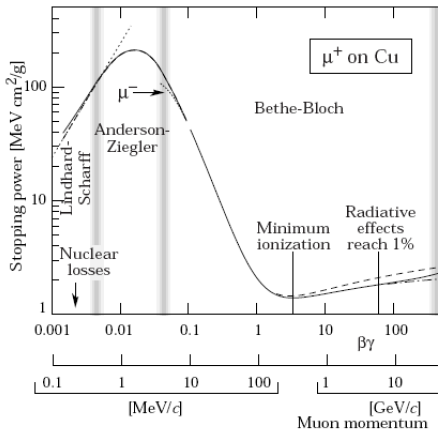
\includegraphics[width=0.7\linewidth]{IMG/ch1/MassicStoppingPower}
	\caption{Massic stopping power as a function of the $\mu^+$ momentum passing through a copper layer~\cite{PDG}.}
	\label{fig:massicstoppingpower}
\end{figure}
\noindent In the trend of the stopping power as a function of the momentum it can be noted a de-growth for low momentum values that is due to the term $\frac{1}{\beta^2}$ in equation \ref{eq:bethe}; the stopping power decreases until it reaches a minimum, and then slowly grows back.
\newline
The average path (range) of a charged particle can be calculated by integrating the stopping power along the "walk".
\begin{equation}\label{eq:range}
	R=\int_{E_i}^{0} \frac{1}{\frac{dE}{dx}}dx
\end{equation}
\noindent The range depends approximately on the A / Z ratio of the material and increases approximately with the square of the initial kinetic energy of the charged particle.
The energy loss rate increases as the kinetic energy of the particle decreases with the depth of penetration, with a rapid ascent at the end of the path.
The density of ionization of the charged particles along their path in the medium is therefore characterized by a plateau followed by a pronounced maximum towards the end of range, called Bragg peak, which is located at a depth depending on the initial energy of the incident particle, as shown in figure \ref{fig:braggpeak}.
\newline
If more particles are considered then it should be kept in mind
the statistical fluctuations on the collisions of the particles and on the energy transferred for each collision.
These fluctuations, well described by the Landau distribution~\cite{landau}, generate uncertainty about the distance reached by the particles ("straggling").
Beyond all these considerations we must also take into account the possible interactions with the nuclear components of the matter crossed.
One effect is lateral enlargement of the beam due to the Multiple Coulomb Scattering (MCS) interaction of the nuclei that it is inversely proportional to the mass of the incident particle.
The second effect is due to the fragmentation of the primary bundle and/or of the nuclei of the passed-though material due to nuclear interactions.
The fragmentation cross section becomes relevant for ions heavier than the proton, such as carbon ions or heavier, and causes a decrease in the number of particles incident along the path and the development of secondary fragments.
The fragments produced deposit theirs energy deeper than the Bragg peak giving rise to a queue in the distribution.
\begin{figure}[H]
	\centering
	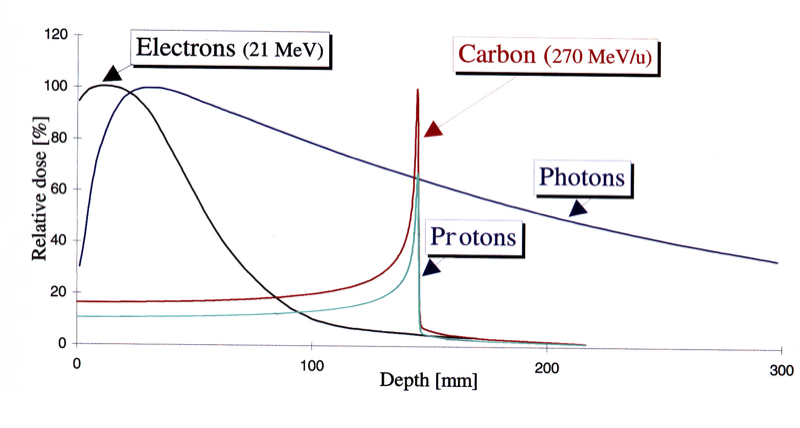
\includegraphics[width=0.8\linewidth]{IMG/ch1/BraggPeak2}
	\caption{Dose profile for a 21~MeV electron, 270~MeV/u carbon ion and photon beam~\cite{bragg}.}
	\label{fig:braggpeak}
\end{figure}  


\section{Effects of radiations on biological systems}
Radiation is energy.
When a charged particle interacts with the human body it loses its energy.
The measurement and calculation of the ionizing radiation dose absorbed by an object is called radiation dosimetry.
\newline
The dose (D) can be defined as the energy absorbed divided by the object mass.
\begin{equation}\label{eq:dose}
	D\left[Gy \right] =\frac{dE}{dm}
\end{equation}
In the I.S. the unit of measure is the Gray(Gy), with 1~Gy~=~1~J/Kg.
\newline
It is also common the use of an equivalent dose (H=DxW$_1$) where W$_1$ is a weight that depends on the type of particle (photon, electron, neutron, proton, heavy charged particle, etc...). The unit of measure of the equivalent dose is the Sievert(Sv) (1~Sv~=~1~J/Kg), although in the past it was used the rem (1~Sv~=~100~rem).
\newline
When monitoring the dose absorbed by an human body it must be considered that not every organ has the same resistance to radiation, thus it is used the effective dose (E~=~HxW$_2$) which is the equivalent dose multiplied by the weight W$_2$ which depends on the part of the body interested by the radiations.
\newline
\noindent The energy deposition is strictly dependent by the type of radiation like photons, electrons or heavy charged particles. As shown in figure \ref{fig:braggpeak} the relative dose percentage delivered by the photons is maximum at low depth and then has an exponential decrease as the depth in the tissue increases.
The dose profile as a function of the depth for heavy charged particles (as carbon ions) is characterized by a low dose at the beginning of the tissue and then by an extremely peaked spike at the end of their travel (Bragg peak).
Since the depth of this peak depends on the beam energy, this can be tuned to deliver the dose at different depths.
Moreover, thanks to the high mass of the particles, it is possible to greatly reduce the lateral diffusion effects thus saving the healthy tissues and the critical structures near the target.
\begin{figure}[H]
	\centering
	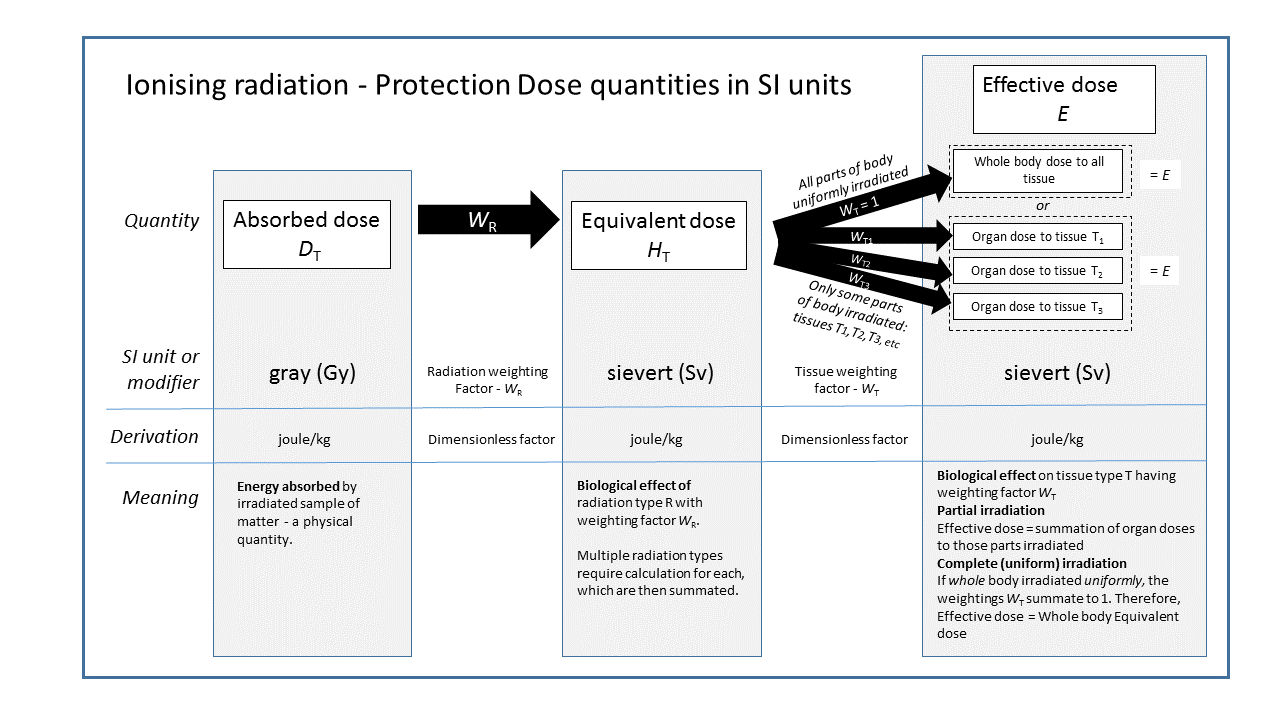
\includegraphics[width=0.7\linewidth]{IMG/ch1/SIRadiationDoseUnits}
	\caption{Absorbed, equivalent and effective dose units and meanings.}
	\label{fig:SIRadiationDoseUnits}
\end{figure} 
\noindent With heavy charged particles it is therefore possible to accurately focus the beam for a selected depth whereas this is not possible with other sources of radiation.
\newline
The different rates of energy loss at different depths for photons and heavy charged particles produce different dose distributions as shown in figure \ref{fig:Dose}, for a single beam direction.
\begin{figure}[H]
	\centering
	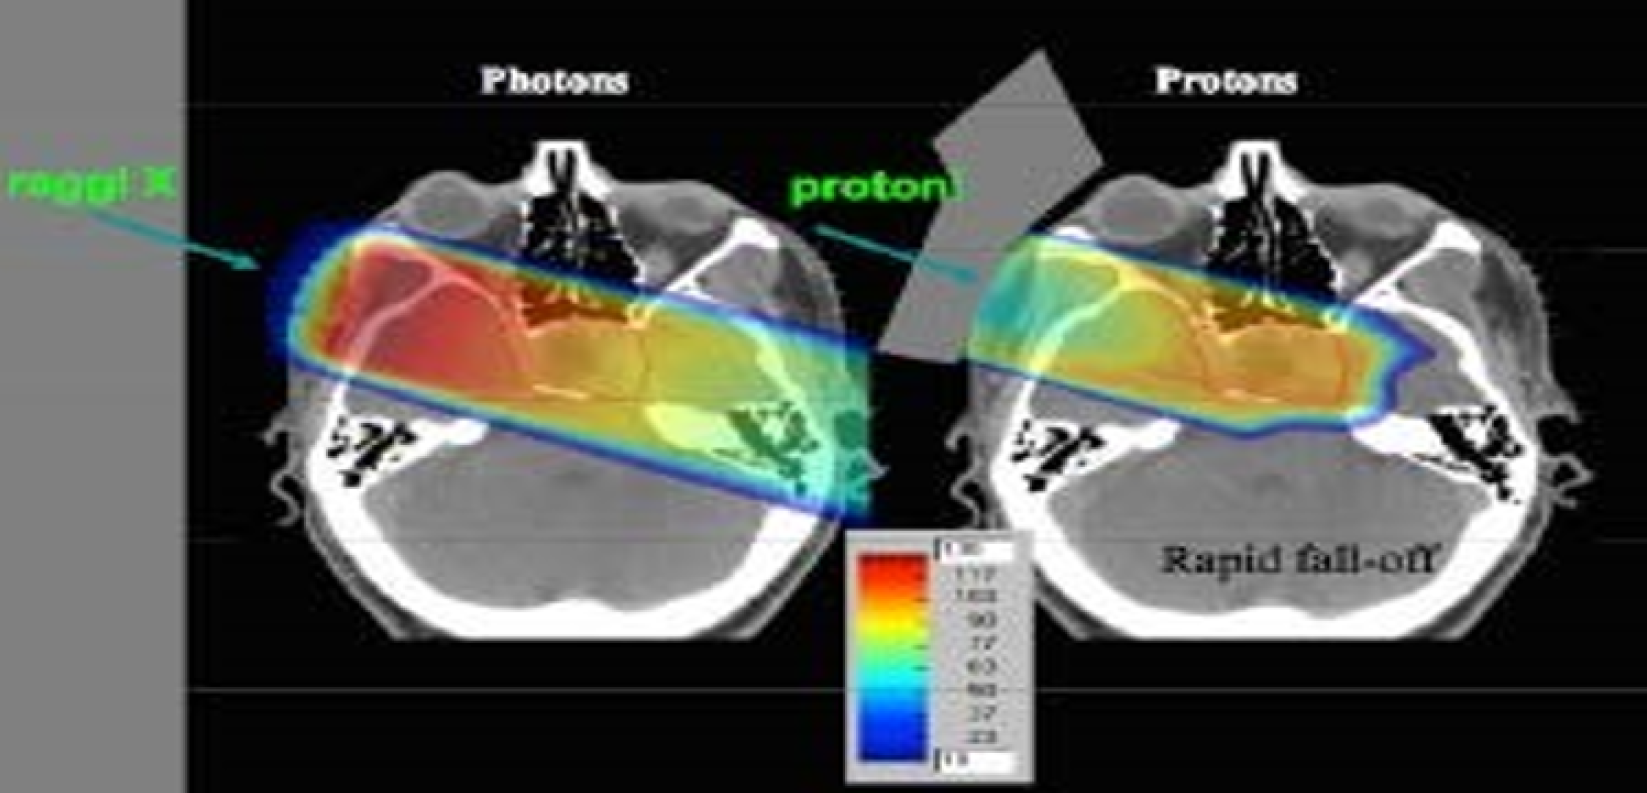
\includegraphics[width=0.7\linewidth]{IMG/ch1/Dose}
	\caption{Example of a dose distribution for a photon beam (left) and for a proton beam (right); to be noted that in a real application the beam is coming from multiple directions in order to minimize the dose delivered to the healthy tissues.}
	\label{fig:Dose}
\end{figure}

\noindent The energy released by the charged particles can cause both direct and indirect effects.
The direct ones are the interactions between the radiation and the biological molecules,
which generate breaking points in the nucleotide chain of the DNA.
The indirect effects are the interactions between radiations and water molecules inside the cell with production of free radicals.
After that the free radicals can diffuse and interact with the biological molecules, producing chemical alterations that can generate the inactivation of the cell cycle.
Damage to DNA molecules is considered the most important effect since it can lead to the cell inability to reproduce and to cell death~\cite{cells}.
\newline
Irradiation can produce various types of alterations in the DNA structure:
\begin{itemize}
	\item \textbf{Single Strand Break} (SSB) when the nucleotide is damaged on a single DNA filament;
	\item \textbf{Double Strand Break} (DSB) when two or more nucleotide are damaged on both DNA filaments. 
\end{itemize}
Following the damage, there are several scenarios:
\begin{itemize}
	\item \textbf{complete repair}, a situation that occurs for the majority of minor alterations (SSB), after which the cell resumes its normal activity;
	\item \textbf{wrong repair}, in which the cell repairs its damage but not comprehensively. This can lead to the impossibility of replication of the cell or to its death by apoptosis. In some cases the cell may be able to divide, but by passing on a genetic mutation;
	\item \textbf{unrepairable damage}, in this scenario the cell dies within a few hours due to the release of lytic enzymes or dies on the occasion of the first mitotic division. This situation occurs mainly in the case of DSB.
\end{itemize}
The cellular response to radiation depends in a complex way on the absorbed dose.
In radiobiology, the biological efficacy of a radiation dose is studied by measuring the cell survival as a function of the dose irradiated on the sample. The main physical factor on which biological damage depends, for the same dose administered, is the Linear Energy Transfer (LET)~\cite{let}:   
\begin{equation}\label{eq:let}
	LET=\frac{dE}{dx}
\end{equation}
\noindent The LTE is defined as the average ionization density along the trail of a particle and is measured in keV/$\mu m$.
Radiations with high LET have, considering fixed the absorbed dose, a greater biological effect compared to the ones with low LET.
This happens because a higher ionization density implies a greater probability of unrepairable damages, like DSB.
The biological effect of a radiation is quantified in terms of Relative Biological Efficiency (RBE), defined as the ratio between the dose required to obtain a specific effect respectively with a reference radiation and with the radiation in question.
\begin{equation}\label{eq:rbe}
	RBE=\frac{D_{ref}}{D_{test}}
\end{equation}
\noindent The reference radiation $D_{ref}$ is commonly represented by a 250 keV X-ray beam, while $D_{test}$ corresponds to the dose of the radiation under examination.
\begin{figure}[H]
	\centering
	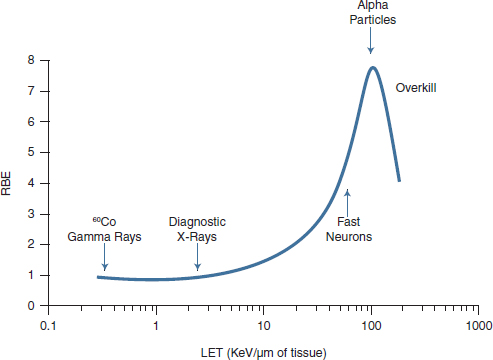
\includegraphics[width=0.7\linewidth]{IMG/ch1/RBE}
	\caption{RBE in function of the LET.}
	\label{fig:rbe}
\end{figure}
\noindent In figure \ref{fig:rbe} it can be seen how the RBE changes as a function of the radiation LET. From the graph it can be noted that the RBE growth, as a function of the LET, starts for values near 1 keV/$\mu m$ and reaches a maximum near 100 keV/$\mu m$. For even higher LET values the RBE decreases; this is caused by a biological saturation effect that happens for high dose (overkill). 
10 MeV carbon ions have a LET of 170 keV/$\mu m$, this correspond to a RBE of 7. This is one of the reasons why therapies based on the use of carbon ions have been developed, which at the same dose, produce greater biological effects and are more effective in the treatment of radio-resistant tumors.


\section{Dose distribution systems in hadron therapy}
The physical and biological advantages of therapies with charged particles described in the previous paragraphs allow to obtain a precise conformation of the dose to the tumor, while minimizing the risk of side effects due to the irradiation of surrounding healthy organs.
These advantages are nowadays exploited in the treatment of delicate tumors in the proximity of organs at risk, pediatric tumors where the risk of side effects must be minimal, and radio-resistant tumors.
The number of patients treated with protons or carbon ions is growing each year as it can be seen in figure \ref{fig:patientstreated}.
\begin{figure}[H]
	\centering
	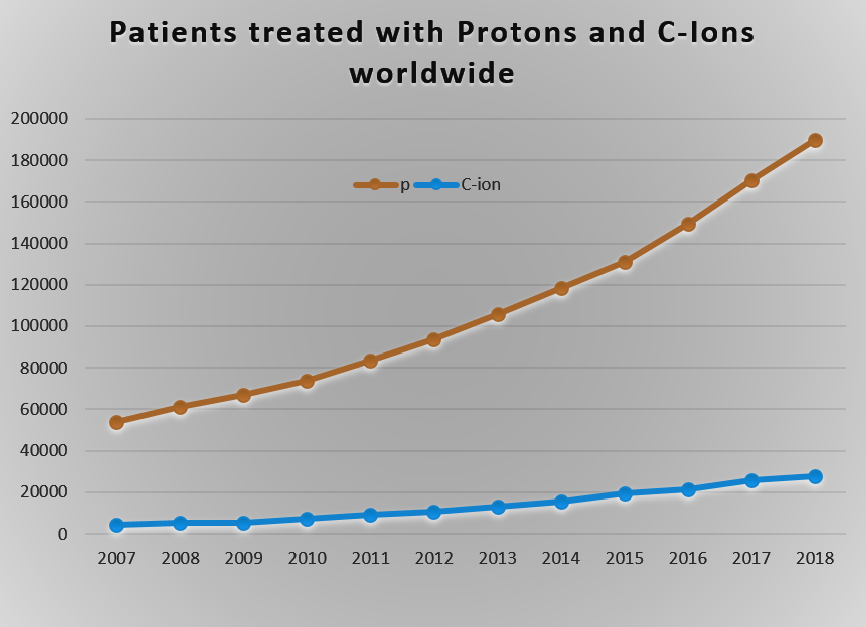
\includegraphics[width=0.7\linewidth]{IMG/ch1/PatientsTreated2}
	\caption{Number of patients treated annually with protons and carbon ions~\cite{world}.}
	\label{fig:patientstreated}
\end{figure}
\noindent This numbers, even if growing, are still a small fraction of the total number of tumors treated with external radiation, being X-ray the main therapy method. 
The main reason lies in the need for complex accelerators (cyclotrons or synchrotrons) to accelerate the ions to
the energies needed to penetrate deeply into the tissues and a sophisticated dose distribution system that guarantees the achievable precision in delivering the dose in the various regions of the patient.
\newline
Cyclotrons take up less space and are cheaper to build and to maintain, however the accelerated particles have fixed energy that can not be changed. It can only be reduced using absorbent elements called range shifter.
On the contrary, a synchrotron can accelerate ions at different energies, but it needs much more space and money to operate.
Typically a medical purpose synchrotron like the one in figure \ref{fig:sincrotrone} has a ring of at least 10m in diameter and needs one or two linear accelerators in series to inject the particles in the main ring.
\begin{figure}[H]
	\centering
	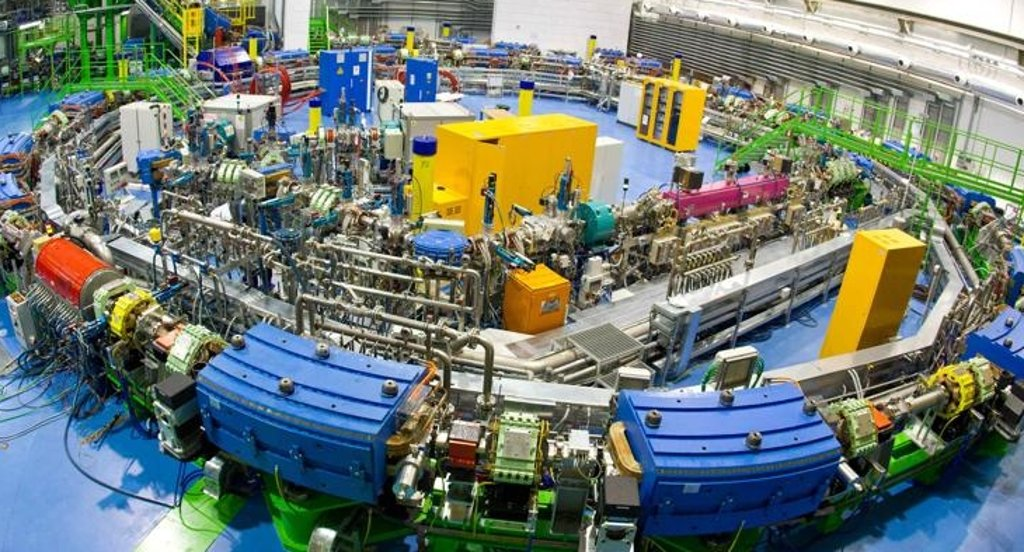
\includegraphics[width=0.7\linewidth]{IMG/ch1/Sincrotrone}
	\caption{The synchrotron at the National Center of Oncological Hadrotherapy (CNAO) of Pavia.}
	\label{fig:sincrotrone}
\end{figure}
\noindent Regardless of the type of acceleration used, it is crucial that the beam remains modulated in energy and direction in such a way to produce an optimal dose distribution. This is generally achieved by producing a Spread Out Bragg Peak (SOBP), a constant longitudinal dose distribution in the volume to be treated obtained by superimposing beams at different energies, as shown in figure \ref{fig:sobp}.
\begin{figure}[H]
	\centering
	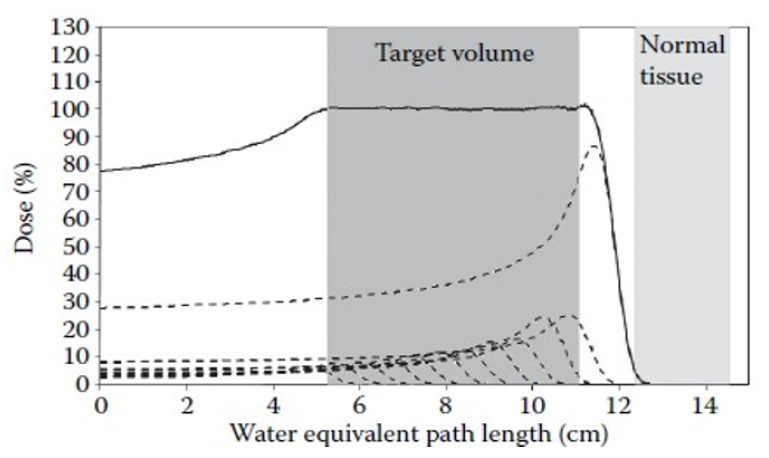
\includegraphics[width=0.7\linewidth]{IMG/ch1/SOBP}
	\caption{The SOBP is obtained by superimposing multiple beams with different energy, thus creating a dose profile constant with the depth of the tissue~\cite{sobp}.}
	\label{fig:sobp}
\end{figure}
\noindent There are two ways to conform the particle beam to the volume to be treated, these are passive and active distribution systems.

\subsection{Passive dose distribution systems}
\noindent Passive dose distribution techniques are mainly employed in centers where a cyclotron is used, which provides a fixed energy beam.
The passive methods consist in the use of appropriate absorbing and collimating elements that cause a broadening of the beam, modify its energy in order to produce an appropriate SOBP and adapt the lateral shape to the volume to be treated.
\begin{figure}[H]
	\centering
	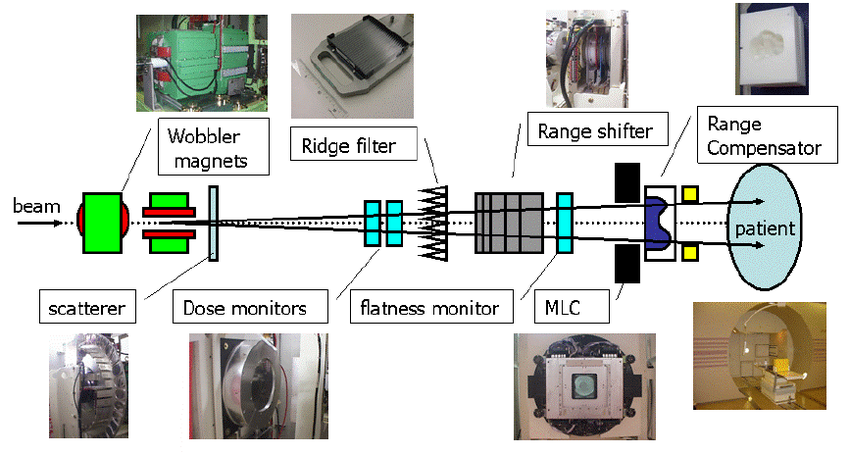
\includegraphics[width=0.9\linewidth]{IMG/ch1/Basic-design-of-irradiation-system-for-hadron-therapy}
	\caption{Basic design of passive dose distribution system for hadron therapy used to adapt the dose to the form of the tumor.}
	\label{fig:passive}
\end{figure}
\noindent A typical example of a passive dose distribution system is shown in figure \ref{fig:passive}.
A fixed energy beam passes through a first thin layer of scattering material (scatter), such as lead, that causes the beam to broaden with a simil-gaussian transverse distribution.
The thin thickness of the material means that the energy loss is minimum.
The dose is monitored with some ionization chambers.
The maximum energy and thus the SOBP is set with the use of range shifters.
The beam lateral profile is adapted to the form of the tumor with the use of collimators.
The dose is set in accordance with the shape of the tumor with the use of range compensators.
\newline
The advantages of this technique are the simplicity, safety, wide diffusion in existential hadrontherapy centers and low sensitivity to the temporal dynamics of the beam. 
On the other hand there is the reduced flexibility in the three dimensional conformation of the dose, the need to use customized collimators, the difficulty of obtaining a truly parallel beam, the low efficiency of use of the beam and the additional dose to the patient due to the production of secondary fragments (for example neutrons) in nuclear interactions with absorbent elements.

\subsection{Active dose distribution systems}
\noindent Unlike passive systems in which the beam is spread to cover the entire tumor area, in active distribution systems the tumor volume is divided into a grid of points, called spots, that are grouped into several mono-energetic layers, where each layer corresponds to the position of the Bragg peak of a narrow, fixed energy beam, called pencil beam.
The lateral conformation is obtained with a magnetic deflection, while the energy of the beam is changed to move the Bragg peak from one layer to the other.
In active systems based on cyclotrons, the energy of the beam is changed using absorbent materials (range shifters) of appropriate thickness, followed by magnetic energy selection systems, while in synchrotron-based centers, directly changing the energy at which the beam is accelerated between one spill and the next.
Scanning in the direction orthogonal to the beam is performed with two perpendicular magnets.
\newline
There are two modes of active distribution. In one the beam is moved continuously along the scanning lines and the transverse dose distribution is modulated by adjusting the scanning speed (raster scanning). A second mode (spot scanning)~\cite{cnao} consists in keeping the beam fixed on a spot until the predetermined dose is reached, and then moving it, without turning it off, to the adjacent spot until the whole mono-energetic slice is completely irradiated, as shown in figure \ref{fig:active}.
\begin{figure}[H]
	\centering
	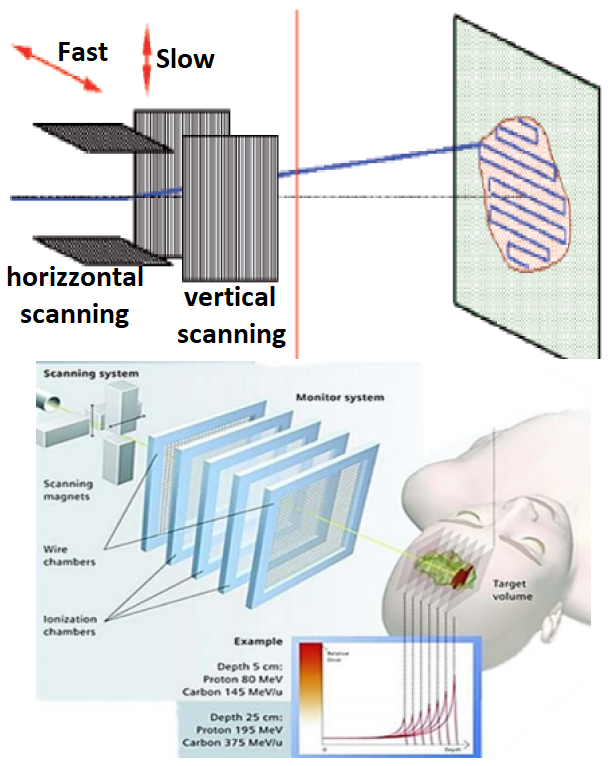
\includegraphics[width=0.7\linewidth]{IMG/ch1/Active2}
	\caption{Basic design of active dose distribution system for hadron therapy used to adapt the dose to the form of the tumor. Dose distribution in the transverse plane is modulated by scanning magnets (top) and on the longitudinal axis with the superposition of energy beams different (bottom).}
	\label{fig:active}
\end{figure}
\noindent The second technique provides the enormous advantage of being able to perform an extremely precise and homogeneous irradiation that adapts to the shape of the tumor, which is in most cases irregular, without the use of patient-specific passive elements.
Another advantage compared to passive systems is the absence of material on the beam line, a lower lateral penumbra due to the absence of collimators, a high efficiency in the use of the beam and the possibility to synchronize the radiation with the respiratory phase of the patient.

\subsection{Treatment Planning System}
\noindent The Treatment Planning System (TPS) is a software that simulates the patient dose distribution and calculates the optimal beam configuration to achieve clinical dose specifications for the tumor and healthy organs.
It is a complex tool, which uses information on the patient's anatomy as input provided by computed tomography (CT) images, with physician-designated contours of the tumor and surrounding organs.
Based on this information and on the specifications of the desired target dose and the maximum tolerable dose on other organs, the TPS performs a minimization procedure (called "reverse planning") to determine the treatment parameters.
The output of the TPS provides the parameters corresponding to the number of particles, energies and directions of the pencil beam for each spot necessary to best meet the specifications.
The TPS searches for the solution iteratively: starting from an initial hypothesis on the number of particles for each spot, the program calculates the spectra of the particles for each point of interest and estimates the corresponding biological effect.
If the result meets the specifications, the TPS can terminate the execution while if not the program must appropriately vary the number of irradiated particles and repeat the biological effect assessment, until the specifications are met or the maximum number of iterations is reached.


\section{Beam monitoring}
\noindent The accuracy of the dose distribution obtained with the active pencil beam scanning technique is based on a precise online measurement of the beam position and the number of particles irradiated at each point.
The Dose Distribution System (DDS)~\cite{pencil} must control the scanning system, consisting of two power supplies connected to two orthogonal bipolar magnets to deflect the beam horizontally and vertically.
Once the required number of particles are irradiated in one spot, the DDS changes the currents in the magnets in order to move the beam to the next point.
Moreover, the DDS must be interfaced with the accelerator control to request a quick stop of the beam when a slice is completed or to request a new energy value for the treatment of the next slice.
The operations of the DDS are all based on the online measurement of the number of irradiated particles and the direction of the beam carried out with dedicated detectors.
\subsection{Ionization chambers}
The most commonly used monitor detectors are based on ionization chambers.
figure \ref{fig:monitor}, for example, shows the beam detector system used by the National Center of Oncological Hadrotherapy (CNAO) in Pavia, consisting of five planar ionization chambers filled with nitrogen and positioned at the end of the beam line.
Two chambers with a single electrode provide information on the number of particles irradiated with a frequency of 1~MHz, while the other three chambers have electrodes segmented into strips or pixels for measuring the shape and position of the beam.
\newline
\noindent Due to their limited complexity, ionization chambers offer several advantages such as robustness, ease of construction and operation, and show no indication of performance degradation due to radiation and aging effects, even after several years of operation.
Despite being the gold standard in beam monitoring applications in hadrontherapy, the imminent development of new treatment techniques are beginning to suffer from the limitations of gas detector technology.
\newline
Ionization chambers measure the charge produced in the gas, which depends not only on the number of particles, but also on the energy of the particles and environmental parameters.
To determine the number of particles irradiated on each spot, the energy of the beam must be known in advance as well as the effects of temperature and pressure dependencies must be taken into account.
Periodic calibration procedures are required to ensure the reliability of the ionization chambers in clinical practice.
Another limitation of the ionization chambers is their limited sensitivity: due to the small ionization charge produced in gases, the minimum number of particles that an ionization chamber can detect is limited to about $10^4$ protons.
Furthermore, the collection times of the charge in the gas are relatively long (of the order of hundreds of $\mu$s) and therefore their response is rather slow.
These limitations prevent their use in treatment modalities where rapid changes in position are required or when a limited number of particles must be irradiated at each spot.
\begin{figure}[H]
	\centering
	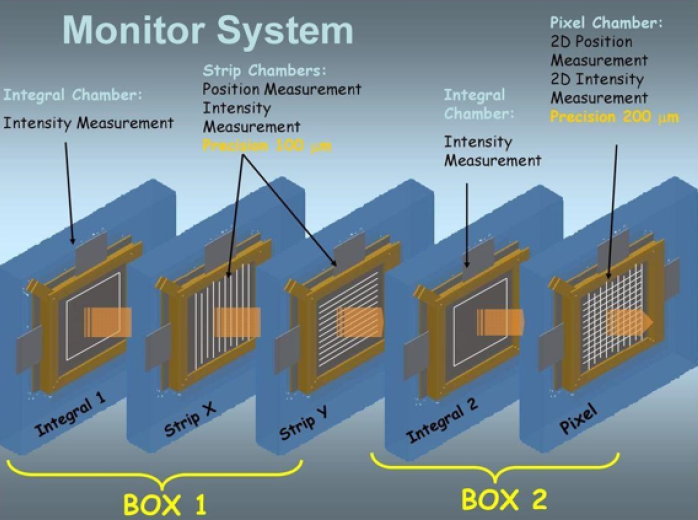
\includegraphics[width=0.7\linewidth]{IMG/ch1/MonitorSystem.PNG}
	\caption{Ionization chamber diagram.}
	\label{fig:monitor}
\end{figure}
\noindent To overcome the limitations of ionization chambers as monitoring devices in hadrontherapy, as their limited sensitivity, the dependence of the measurable number of particles on the energy of the beam and environmental parameters, slow response times, the Medical Physics group of the University of Turin is studying a new approach for beam monitoring based on solid state detectors.
In particular, segmented silicon detectors are considered as an alternative to ionization chambers to count the number of particles in a therapeutic beam.
\newline
In the next paragraph it is described the operation of a silicon detector, while in the next chapter it will be shown how their characteristics can compensate for the limitations of the ionization chambers.

\subsection{Silicon detectors}

\noindent Silicon is a semiconductor formed by tetravalent atoms~\cite{detector}, with a resistivity between that of the metal and the insulators, with a forbidden energy band of 1.14 eV.
An electron jumping in the conduction band leaves a hole in the valence band, which behaves like a positive charge carrier.
When silicon is doped with trivalent atoms (acceptors) there is an excess of holes ("p-type" material).
Doping with pentavalent (donor) atoms produces materials with an excess of electrons (called "n-type").
\newline
A silicon detector is based on p-n junctions, and on the formation of a depletion region without free charges obtained by applying an intense reverse polarization.
In a silicon detector the depletion region is the active volume in which the hole-electron pairs are created by the ionization of the particles, similar to how ion-electron pairs are produced in a gas detector.
The current induced in the electrode during the migration of the hole-electron pairs is collected and integrated to measure the total charge produced, proportional to the loss of energy by the charged particle.
\newline
The average energy required to create a hole-electron pair is an order of magnitude smaller in silicon than in a gas (3.6 eV in Si compared to more than 30~eV in N$_2$ or in air).
Also considering the much higher density of silicon than a gas, the charge produced by a ionizing particle in a thin layer of silicon is high enough to be measurable even for a single particle.
\newline
The silicon detectors are constructed with a series of p-n junctions with the electrodes segmented into strips or pixels, and used for particle monitoring in particle physics and nuclear physics applications.
An example of a silicon strip detector is shown in figure \ref{fig:detector}. It consists of highly doped p-type strips implanted on an n-type substrate and an n ++ electrode.
The substrate n is completely depleted by applying a positive voltage on the electrode n++ with respect to the strips.
A ionizing particle penetrates the depleted substrate and generates electron-hole pairs that migrate along the electric field generated by the applied voltage and induces a current signal on the aluminum strips.
In this example, the aluminum electrodes are separated by a thin SiO2 capacitive layer (AC coupling), but configurations with direct connection of the aluminum to the n ++ electrode (DC coupling) are also possible.
In a typical strip detector, the thickness of the depleted region is about 300~$\mu$m to produce a sufficient charge detectable by the subsequent read-out electronics. 
The typical collection time of electrons and holes varies from 3~ns to 6~ns, depending on the applied voltage.
\begin{figure}[H]
	\centering
	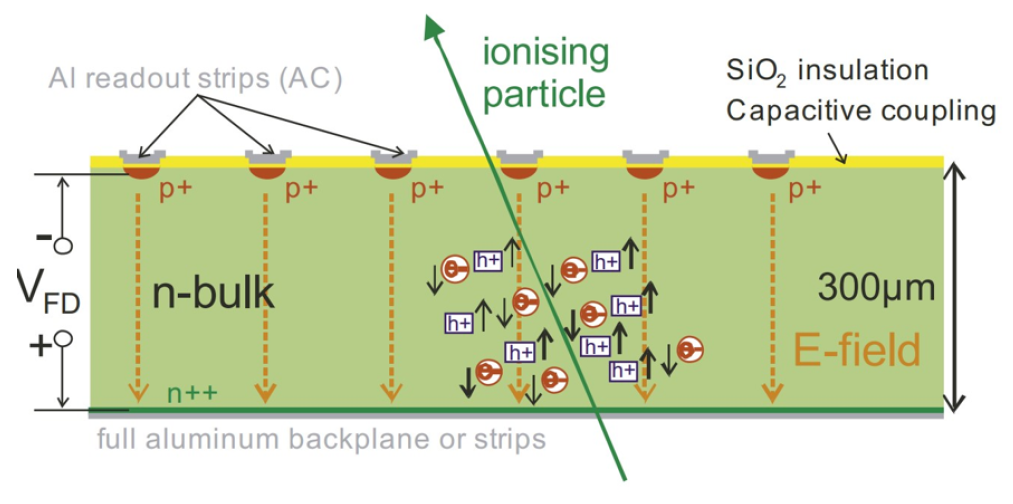
\includegraphics[width=0.7\linewidth]{IMG/ch1/Detector.PNG}
	\caption{Schematic of a silicon detector with strip segmented electrodes~\cite{detector}.}
	\label{fig:detector}
\end{figure}
